\section{Aufgabe 1}
\subsection{Bestimmung der Federkonstanten}
Die Federkonstante $k$ einer Feederwaage soll nach dem Hookschen Gesetz
\begin{equation}
F = k \cdot x
\label{eqn:hookeq}
\end{equation}
bestimmt werden. Hierzu werden verschiedene Gewichte $m$ an die Federwaage gehängt und die jeweilige Ausdehnung $x$ 
gemessen. Diese Messwerte sind in der Tabelle \ref{tab:gemDaten} angegeben.

\begin{table}
\centering
\caption{Gemessene Auslenkungen bei verschiedenen Massen.}
\label{tab:gemDaten}
\begin{tabular}{c c}
    $m [\symup{g}]$ & $x [\symup{cm}]$ \\
    \midrule
    2 & 1.6 \\
    3 & 2.7 \\
    4 & 3.2 \\
    5 & 3.5 \\
    6 & 4.0 \\
    \bottomrule
\end{tabular}
\end{table}
Für die Bestimmung einer linearen Ausgleichsgerade wird die Beziehung
\begin{equation}
x = a \cdot m + b
\label{eqn:ausglgeradetheorie}
\end{equation}
verwendet. Hierbei gilt für $a$
\begin{equation}
a = \frac{g}{k}
\label{eqn:beschl}
\end{equation}
wobei $g$ die Schwerebeschleunigung $g = \SI{9.81}{\meter\per\second\squared}$ ist.

\subsection{m-x Diagramm}
\begin{flushleft}
Zuerst lässt sich mit Python und der Bibliothek \enquote{matplotlib} die Abbildung \ref{fig:plot1} erstellen.\\
Nun lässt sich eine Ausgleichsgerade finden, dabei wird die Methode der kleinsten Quadrate angewendet. Dazu müssen folgende Gleichungen gelöst werden.
\end{flushleft}

\begin{minipage}{0.4\textwidth}
\begin{equation}
a = {{\overline{m \cdot x} - \overline{m}\cdot
    \overline{x}} \over {\overline{m^2} - {\overline{m}}^2}}
\label{eqn:aeq}
\end{equation}
\end{minipage}
\begin{minipage}{0.4\textwidth}
\begin{equation}
b = {{\overline{m^2} \cdot \overline{x} -    \overline{m} \cdot {\overline{m \cdot x}}}\over{\overline{m^2} -    {\overline{m}}^2}}
\label{eqn:beq}
\end{equation}
\end{minipage}

\begin{flushleft}
Diese Größen sind allerdings auch fehlerbehaftet und es muss die Standardabweichung auf \eqref{eqn:aeq} und \eqref{eqn:beq} berechnet werden.
$\sigma_a^2$ beschreibt den Schätzer der Varianz für $a$, und $\sigma_b^2$ den Schätzer der Varianz für $b$.
\end{flushleft}
\begin{minipage}{0.45\textwidth}
\begin{equation}
\sigma_a^2 = \frac{S_{x|m}^2}{\sum_{i=1}^n (m_i - \overline{m})^2}
\label{eqn:standarderrora}
\end{equation}
\end{minipage}
\begin{minipage}{0.45\textwidth}
\begin{equation}
\sigma_b^2 = \frac{S_{x|m}^2}{n} \frac{\sum_{i=1}^n m_i^2}{\sum_{i=1}^n (m_i - \overline{m})^2}
\label{eqn:standarderrorb}
\end{equation}
\end{minipage}

\begin{flushleft}
$S_{x|m}^2$ ist hier die Residualvarianz
\end{flushleft}
\begin{equation}
S_{x|m}^2 = \frac{1}{n-2} \sum_{i=1}^n (x_i - (b + a m_i))^2 = 0.068
\end{equation}
%\begin{flushleft}
%Mit den Messwerten können nun die folgenden Werte ausgerechnet werden
%\end{flushleft}
%
%\begin{minipage}{0.4\textwidth}
%\begin{equation}
%\overline{m} = \frac{1}{n} \sum_{i=1}^n m_i = 4
%\end{equation}
%\end{minipage}
%\begin{minipage}{0.4\textwidth}
%\begin{equation}
%\overline{x} = \frac{1}{n} \sum_{i=1}^n x_i = 3
%\end{equation}
%\end{minipage}
%\begin{flushleft}
%~
%\end{flushleft}
%\begin{minipage}{0.45\textwidth}
%\begin{equation}
%\overline{m^2} = \frac{1}{n} \sum_{i=1}^n m_i^2 = 18
%\end{equation}
%\end{minipage}
%\begin{minipage}{0.45\textwidth}
%\begin{equation}
%\overline{m}^2 = \left( \frac{1}{n} \sum_{i=1}^n m_i \right)^2 = 16
%\end{equation}
%\end{minipage}
%\begin{flushleft}
%~
%\end{flushleft}
%\begin{minipage}{1\textwidth}
%\centering
%\begin{equation}
%\overline{mx} = \frac{1}{n} \sum_{i=1}^n m_i x_i = 13.12
%\end{equation}
%\end{minipage}
\begin{figure}[t]
  \centering
  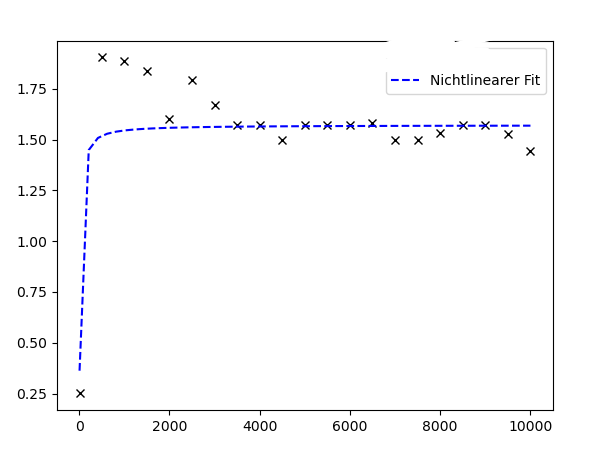
\includegraphics[width=\textwidth]{build/plot1.pdf}
  \caption{Messdaten zur Bestimmung der Federkonstante.}
  \label{fig:plot1}
\end{figure}
\begin{flushleft}
Durch einsetzen der gemessenen Werte oder durch den direkten linearen Fit in Python folgen die Ergebnise für $a$ und $b$, sowie jeweils die Fehler zu
\end{flushleft}
\begin{equation}
a = 0.560 \pm 0.082
\end{equation}
\begin{equation}
b = 0.760 \pm 0.350
\end{equation}
\begin{flushleft}
Eine mögliche Ausgleichsgerade wäre also
\end{flushleft}
\begin{equation}
x(m) = 0.56m + 0.76
\end{equation}
\begin{flushleft}
Es lässt sich leicht erkennen, dass die Werte in der richtigen Größenordnung liegen, da die eingezeichnete Gerade in Diagramm \ref{fig:plot2} gut zu den Werten passt. 
\end{flushleft}
\begin{figure}
  \centering
  \includegraphics{build/plot2.pdf}
  \caption{Messdaten mit Ausgleichsgerade.}
  \label{fig:plot2}
\end{figure}
\begin{flushleft}
Die berechneten Werte können mit einem Polyfit ersten Grades in Python leicht auf ihre Richtigkeit überprüft werden.
Nun lässt sich auch der Wert für die Federkonstante $k$ berechnen. Die Berechnung sieht folgendermaßen aus
\end{flushleft}
\begin{align}
k &= \frac{g}{a} &&= \frac{981\si[per-mode=symbol]{\centi\meter\per\second\squared}}{0.56\si[per-mode=symbol]{\centi\meter\per\gram}} &&= 1751.8\si[per-mode=symbol]{\gram\per\second\squared} \\
\increment k &= \Bigl| \frac{\dif{k}}{\dif{a}} \Bigr| \cdot \increment a &&= \frac{981\si[per-mode=symbol]{\centi\meter\per\second\squared}}{(0.56\si[per-mode=symbol]{\centi\meter\per\gram})^2} \cdot 0.082\si[per-mode=symbol]{\centi\meter\per\gram} &&=  256.5\si[per-mode=symbol]{\gram\per\second\squared}
\end{align}
\begin{flushleft}
Also ergibt sich die Federkonstante mit ihrem Fehlerintervall zu
\end{flushleft}
\begin{equation}
k = \SI{1751{,}8(2565)}{\gram\per\second\squared}
\end{equation}


